\documentclass[../main.tex]{subfiles}

\begin{document}
    
    \chapter{Real Business Cycle Model}
    
    \section{Stylized facts}
    \textbf{Business-Cycle Facts}
    \begin{itemize}
    
        \item
        Fluctuations do not exhibit any simple regular or cyclical pattern
        
        \item
        Output declines and their patterns vary considerably in size and spacing
        
        \item
        Fluctuations are distributed very unevenly over the components of output
        
        \item
        Output growth is distributed roughly symmetrically around its mean, but periods of extremely low growth quickly followed by extremely high growth are much more common than periods exhibiting the reverse pattern
        
        \item
        During recessions:
            \begin{itemize}
            
                \item
                employment falls and unemployment rises
                
                \item
                length of the average workweek falls
                
                \item
                productivity output per worker-hour almost always declines
                
                \item
                real wage tends to fall slightly
                
            \end{itemize}
            
    \end{itemize}
    
    \section{Production with real shocks}
        
        
        Large number of identical competitive (price-taking) firms produce $Y_t$ in period $t$,
        \begin{align}
            Y_t &= K_t^\alpha \left( A_t L_t\right)^{1-\alpha}, \quad \alpha \in (0, 1),
            \\
            &= I_t + C_t + G_t
        \end{align}
        
        where capital $K_t$, technology $A_t$, and labor $L_t$ are production factors. Output $Y_t$ is allocated between investment $I_t$, household consumption $C_t$, and government spending $G_t$. \textbf{Capital $K_t$}, with depreciation rate $\delta$, follows the law of motion
        \begin{align}
            K_{t+1} &= K_t - \delta K_{t} + I_t \\
            &= (1 - \delta) K_{t} + (Y_t - C_t - G_t)
        \end{align}
        
    \subsection{Real Shocks}
        
        \textbf{Technology} follows the law of motion
        \begin{align}
            \ln(A_t) &= \bar{A} + gt + \tilde{A}_t
            \\
            \implies
            A_t
            &= e^{\bar{A} + \tilde{A}_t}e^{gt},
            \quad \frac{\dot{A}_t}{A_t}
            = g + \frac{\dot{\tilde{A}}_t}{\tilde{A}_t},
        \end{align}
        where $\tilde{A}_t$ is a AR(1) process ``technology shock"
        \begin{align}
            \tilde{A}_{t} = \rho_A \tilde{A}_{t-1} + \varepsilon_{A, t},
            \quad \rho_A \in (-1, 1),
            \quad \E{\varepsilon_{A, t}} = 0.
        \end{align}
        
        and $\varepsilon_{A, t}$ are independently and identically distributed (i.i.d.) across periods.
        
        \vspace{0.5cm}
        
        \textbf{Government spending} is financed by lump-sum taxes on production that equal to spending each period (so taxes do not impact model\footnote{Government imposes lump-sum taxes $T_t = G_t$, then after tax output is $Y_t - T_t = C_t + I_t + G_t - T_t = C_t + I_t$.}), and follows the law of motion
        \begin{align}
            \ln(G_t) &= \bar{G} + (n + g)t + \tilde{G}_t,
            \\
            \tilde{G}_t &= \rho_G \tilde{G}_{t - 1} + \varepsilon_{G, t},
            \quad \rho_G \in (-1, 1),
        \end{align}
        and $\E{\varepsilon_{G, t}} = 0$ and are i.i.d. across time.
        
        \vspace{0.5cm}
        
        Perfectly competitive firms maximize profits in each period, 
        \begin{align}
            \Pi_t = Y_{t} - w_t L_t - (r_t + \delta_t) K_t.    
        \end{align}
        
        First order conditions imply factor costs are equal to marginal products,
        \begin{align}
            \frac{\partial \Pi_t}{\partial L_t} = 0
            &\implies
            w_t
            = \frac{\partial Y_t}{\partial L_t} = (1-\alpha) \left(\frac{K_t}{A_t L_t}\right)^\alpha,
            \label{eqn:wage}
            \\
            \frac{\partial \Pi_t}{\partial K_t} = 0
            &\implies
            r_t
            = \frac{\partial Y_t}{\partial K_t} = \alpha \left(\frac{A_t L_t}{K_t}\right)^{1-\alpha}.
            \label{eqn:interest}
        \end{align}
        
    \section{Households}
        
        Let $N_t$ be the population in $H$ identical households. Member per household is then $N_t / H$. Population grows exogenously at a constant continuous rate:
        \begin{align}
            \ln N_t &= \bar{N} + nt
            \implies
            N_t = e^{\bar{N}}e^{nt}. \label{eqn:population}
        \end{align}
        
        Per capita consumption and labor is
        \begin{align}
            c_t &= \frac{C_t}{N_t}, \quad
            \ell_t = \frac{L_t}{N_t} \in [0, 1],
        \end{align}
        
        where labor $\ell_t$ is normalized to percentage of time endowment, and leisure per capita is defined as $1-\ell_t$. The representative individual's instantaneous utility is given by
        \begin{align}
            u_t(c_t, \ell_t) = \ln c_t + b \ln(1-\ell_t),
            \quad b > 0,
        \end{align}
        
        where each period is discounted by the parameter $\rho > n$. Altogether, the \textbf{representative household} (with $N_t/H$ members) maximizes expected utility
        \begin{align}
            & U = \sum_{t=0}^\infty e^{-\rho t}
            \bigg( \ln c_t + b \ln(1-\ell_t) \bigg)
            \frac{N_t}{H}
            \\
            & \qquad\qquad\qquad
            s.t. \nonumber
            \\
            & \sum_{t=0}^{\infty}
            \frac{c_t}{\prod_{s=1}^{t}(1+r_s)} \frac{N_t}{H}
            \le
            \sum_{t=0}^{\infty}
            \frac{w_t \ell_t}{\prod_{s=1}^{t}(1+r_s)} \frac{N_t}{H}.
        \end{align}
        
        Form the Lagrangian
        \begin{align}
            \L
            = \sum_{t=0}^\infty e^{-\rho t}
            \bigg( \ln c_t + b \ln(1-\ell_t) \bigg)
            \frac{N_t}{H} 
            + \lambda \left(
                \sum_{t=0}^{\infty}
                \frac{w_t \ell_t - c_t}{\prod_{s=1}^{t}(1+r_s)}\frac{N_t}{H}
                \right)
        \end{align}
        
        and we have the following FOC for each period $t$ that
        \begin{align}
            \frac{\partial \L}{\partial c_t} = 0
            &\implies
            \frac{1}{c_t}\frac{N_t}{H}e^{-\rho t}
            = \frac{\lambda}{\prod_{s=1}^{t}(1+r_s)} \frac{N_t}{H}, 
            \label{eqn:foc-1}
            \\
            \frac{\partial \L}{\partial \ell_t} = 0
            &\implies
            \frac{b}{1 - \ell_t}\frac{N_t}{H}e^{-\rho t}
            = \frac{\lambda w_t}{\prod_{s=1}^{t}(1+r_s)}\frac{N_t}{H}.
            \label{eqn:foc-2}
        \end{align}
        
        
        Combining the above for two periods $t$ and $t+1$, we have the Euler equations:
        \begin{align}
            \frac{c_{t+1}}{c_t}
            &= e^{-\rho}(1+r_{t+1}),
            \label{eqn:euler-c}
            \\
            \frac{1-\ell_{t+1}}{1-\ell_t}
            &= e^{-\rho}(1+r_{t+1})\frac{w_t}{w_{t+1}}
            \label{eqn:euler-ell}
        \end{align}
        See Appendix~\ref{app:euler-c-ell} for details of derivations. Suppose that
        
    \section{Uncertainty}
    
        By  \eqref{eqn:wage} and \eqref{eqn:interest}, future equilibrium wages $w_t$ and interest rates $r_t$ are uncertain, as they depend on $A_t$ which has a stochastic component. At period $t$,
        the expected utility continuation utility is
        \begin{align}
            U_t &= \Et{\sum_{s=0}^\infty e^{-\rho (t+s)}
            \bigg( \ln c_{t+s} + b \ln(1-\ell_{t+s}) \bigg)
            \frac{N_t}{H}}
            \label{eqn:stoch-utility}
            % \\
            % &= \sum_{s=0}^\infty \left(
            %     \Et{\ln c_{t+s}} + \Et{b \ln(1-\ell_{t+s})}
            % \right)
            % \frac{N_t}{H}e^{-\rho (t+s)}
            \\ s.t. \quad
             & \Et{\sum_{t=0}^{\infty}
             \frac{c_{t+s}}{\prod_{\tau=1}^{{t+1}}(1+r_\tau)}
             \frac{N_t}{H}} \le
            \Et{\sum_{t=0}^{\infty}
            \frac{w_{t+s} \ell_{t+s}}{\prod_{\tau=1}^{{t+1}}(1+r_\tau)}
            \frac{N_t}{H}}.
            \label{eqn:stoch-bc}
        \end{align}
        
        Consider consumption budget of two consecutive periods $t$ and $t+1$. By \eqref{eqn:stoch-bc}, the household consumption budget is
        \begin{align}
            c_{t}\frac{N_{t}}{H} + \Et{\frac{c_{t+1}}{1+r_{t+1}}\frac{N_{t+1}}{H}}
            &= (c_{t} - \Delta c)\frac{N_{t}}{H}
            + \Et{\frac{(c_{t+1} + (1+r_{t+1})e^{-n}\Delta c)}{(1+r_{t+1})} \frac{N_{t+1}}{H}}
            \label{eqn:bc-delta-c}
        \end{align}
        
        Thus, a change of $-\Delta c$ in  $c_t$ should result in a change of $(1+r_{t+1}) e^{-n} \Delta c$ in $c_{t+1}$ within the budget constraint. See Appendix \ref{app:bc-delta-c} for details of the derivation. \\
        
        On the optimal path, allowing changes in $c_t$ and $c_{t+1}$ within the budget constraint, we have the ``stochastic'' Euler equation:
        \begin{align}
            \frac{1}{c_t}
            &= e^{-\rho} \Et{\frac{1+r_{t+1}}{c_{t+1}}}
            \label{eqn:euler-c-stoch}
        \end{align}
        See Appendix \eqref{app:euler-c-stoch} for details.
    
    \section{Optimal consumption-labor choices}
        
        In any period, the one period budget constraint is $dc = \Delta c = w_t \Delta \ell$. Then at the optimal single-period choice we have
        \begin{align}
            d u
            = \frac{\partial u}{\partial c_t} d c_t + \frac{\partial u}{\partial \ell_t} d \ell_t
            = 0
            &= \frac{1}{c_t} dc_t
            - \frac{b}{1 - \ell_t} d\ell_t
            \\
            &= \frac{1}{c_t} w_t \Delta \ell
            - \frac{b}{1 - \ell_t} \Delta \ell
            = 0
            \\
            \implies
            \frac{1}{c_t} w_t \Delta \ell
            &= \frac{b}{1 - \ell_t} \Delta \ell
            \\
            \implies
            \frac{1}{c_t}
            &= \frac{b}{w_t(1 - \ell_t)}.
        \end{align}
        
        Which gives us a relationship for the optimal within-period consumption and labor choice. Then with optimal intertemporal consumption choice in \eqref{eqn:euler-c-stoch}, we have that
        \begin{align}
            \frac{1}{c_t}
            &= e^{-\rho} \Et{(1+r_{t+1})\frac{1}{c_{t+1}}}
            \\ \implies
            \frac{b}{w_t(1 - \ell_t)}
            &= e^{-\rho} \Et{(1+r_{t+1})\frac{b}{w_{t+1} (1-\ell_{t+1})}}
            \\ \implies
            \frac{1}{(1 - \ell_t)}
            &= e^{-\rho} \Et{\frac{ w_t}{w_{t+1}}\frac{1+r_{t+1}}{1-\ell_{t+1}}}.
        \end{align}
    
    
    \section{Model Results}
        
        Baseline model predicts volatility of output, and relative to volatility of consumption, and investment. Labor predictions are less successful in terms of volatility and correlation to GDP per capita.
        
        \begin{figure}[ht!]
            \centering 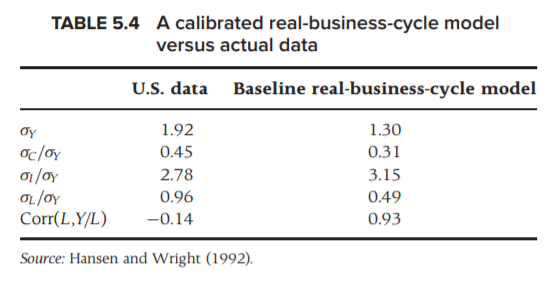
\includegraphics[width=0.6\textwidth]{subfile/attachments/5.3-RBC Empricial Results.png}
        \end{figure}
        
        % Model is solved with numerically. For variable $x$, the impulse response function is defined as
        % \begin{align}
        %     \text{IRF}(h)
        %     = \E{x_{t+h} \lvert \varepsilon_0 = 1}
        %     - \E{x_{t+h} \lvert \varepsilon_0 = 0}.
        % \end{align}
        
        % where $\varepsilon_0$ is the period 0 shock variable in terms of percentage change. A one-period $1 \%$ increase in technology results increases in production via capital. Consumption increases less than output, so savings increase.
        
        




    % appendix
    \renewcommand{\thesection}{A\arabic{chapter}}
    
    \newpage
    \section{Appendix}
    
    \subsection{Euler equation derivations eqs (\ref{eqn:euler-c}) and (\ref{eqn:euler-ell})}\label{app:euler-c-ell}
        
        By FOCs \eqref{eqn:foc-1} and \eqref{eqn:foc-2},
        \begin{align}
            \frac{c_{t+1}}{c_t}
            &= \frac{
                e^{-\rho (t+1)} \left[\prod_{s=1}^{t+1}(1+r_s)\right] / \lambda
                }{
                e^{-\rho t}
                \left[\prod_{s=1}^{t}(1+r_s)\right] / \lambda}
            \\
            &= e^{-\rho}(1+r_{t+1})
            \\
            \frac{1-\ell_{t+1}}{1-\ell_t}
            &= \frac{
                    - b e^{-\rho (t+1)}
                    \left[\prod_{s=1}^{t+1}(1+r_s)\right] / (\lambda w_{t+1})
                    }{
                    - b e^{-\rho t}
                    \left[\prod_{s=1}^{t}(1+r_s)\right] / (\lambda w_t)
                }
            \\
            &= e^{-\rho}(1+r_{t+1})\frac{w_t}{w_{t+1}}
        \end{align}
    
    \subsection{Inter-temporal budget change derivation eq (\ref{eqn:bc-delta-c})}\label{app:bc-delta-c}
        Note that $\frac{N_t}{N_{t+1}} = e^{-n}$ by \eqref{eqn:population}. At period $t$, the present value of  consumption in periods $t$ and $t+1$ is
        \begin{align}
            c_{t}\frac{N_{t}}{H} + \Et{\frac{c_{t+1}}{1+r_{t+1}}\frac{N_{t+1}}{H}}
            &= \left(c_{t}\frac{N_{t}}{H} - \Delta c \frac{N_{t}}{H} \right)+ \Et{ \frac{c_{t+1}N_{t+1}}{(1+r_{t+1})H}} + \Delta c \frac{N_{t}}{H}
            \\
            &= (c_{t} - \Delta c)\frac{N_{t}}{H}
            + \Et{ \frac{c_{t+1}N_{t+1}}{(1+r_{t+1})H}+ \Delta c \frac{N_{t}}{H} }
            \\
            &= (c_{t} - \Delta c)\frac{N_{t}}{H}
            + \Et{\frac{c_{t+1} N_{t+1} + (1+r_{t+1}) \Delta c N_t}{(1+r_{t+1})H}}
            \\
            &= (c_{t} - \Delta c)\frac{N_{t}}{H}
            + \Et{\frac{\left( c_{t+1}
                + (1+r_{t+1}) \frac{N_t}{N_{t+1}} \Delta c \right)}{(1+r_{t+1})}\frac{N_{t+1}}{H}}
            \\
            &= (c_{t} - \Delta c)\frac{N_{t}}{H}
            + \Et{\frac{\left( c_{t+1}
                + (1+r_{t+1}) e^{-n} \Delta c \right)}{(1+r_{t+1})}\frac{N_{t+1}}{H}}
        \end{align}
    
    \subsection{Stochastic Euler equation derivation eq (\ref{eqn:euler-c-stoch})}\label{app:euler-c-stoch}
    
    By \eqref{eqn:bc-delta-c}, a change of $-\Delta c$ in  $c_t$ results in a change of $(1+r_{t+1}) e^{-n} \Delta c$ in $c_{t+1}$ within the budget constraint. On the optimal path, utility remains constant with a slight shift in $c_{t}$ within the budget constraint. Then we have that
    \begin{align}
            d U_t = 0
            &= \frac{\partial U_t}{\partial c_t} dc_t + \frac{\partial U_t}{\partial c_{t+1}} dc_{t+1}
            \\
            &= \frac{1}{c_t}\frac{N_t}{H}e^{-\rho t} dc_t + \Et{\frac{1}{c_{t+1}}\frac{N_{t+1}}{H}e^{-\rho (t+1)} dc_{t+1}}
            \\
            &= \frac{1}{c_t}\frac{N_t}{H}e^{-\rho t} \Delta c + \Et{\frac{1}{c_{t+1}}\frac{N_{t+1}}{H}e^{-\rho (t+1)}  (-(1+r_{t+1})e^{-n}  \Delta c)}
            \\ \implies
            \frac{1}{c_t} \frac{N_t}{H}e^{-\rho t} \Delta c
            &= \Et{\frac{1+r_{t+1}}{c_{t+1}}} \frac{N_{t+1}}{H}e^{-\rho (t+1)}e^{-n} \Delta c 
            \\ \implies
            \frac{1}{c_t}
            &= \Et{\frac{1+r_{t+1}}{c_{t+1}}} \frac{N_{t+1}}{N_t}e^{-n}e^{-\rho} = \Et{\frac{1+r_{t+1}}{c_{t+1}}} e^{-\rho}.
        \end{align}
    
\end{document}